\documentclass{article}
\usepackage[utf8]{inputenc}
\usepackage[T1]{fontenc}
\usepackage{graphicx}
\usepackage{hyperref}
\usepackage{geometry}
\geometry{margin=1in}

\title{Britannica Volume 192984255 Row 473}
\date{Encyclopaedia Britannica (1771)}

\begin{document}
\maketitle

\section*{Historical source}
\textbf{Entry ID:} \texttt{entry-britannica-volume-192984255-row-473-473} \\
\textbf{Volume ID:} 192984255 \\
\textbf{Character Count:} 6693

\subsection*{Extracted Text}
Of the Com Slesa, Misca Madera, were alo fujected to chemical examination, by the fame philosopher. When needed tested best in a crochets, they emitted a perpetraphie fnell of them or feathers, and by further examination, by foliation, the proportion of carbonic matter degraded appeared to be greater, and the proportion of carbonate time lobe, than what was indicated by the refut of the experiments on pencilhenures fields. When natural shells belonging to the fame species, were amended in nitric acid very much diluted, the epidermis separated, and the whole of the carbonate of lime we differed. A gelatinoid diffusence, yearly in a liquid that, remains, ed, but it did not retain the figure of the shell, and ex-philic no appearance at Alorsra Hardure. These fields, therefore, contains a larger portion of gelatinous matter than the porcellaneous fluffs, but the other com-parent part counts entirely of carbonate time.

\_Health composed of nuclear-depart—Shells of this description were subjected to familiar experiments with this former. When the common oyster was expelled to a red heat, the effects were the fans as those which were produced by the fame processis on the facies of patches from Madeira. The foliation of the hallmark shell was also funlier, except only little the gelatinous parts are of a greater confidence. When the river, muffel was burnt a crushing, the melted much make, with a frongu find all burnt born or cartilage; the shell become of a dark gray colour, and exfoliated. By foliation in the acids, the proportion of carbonic matter Separated was greatest, and but of carbonaceous oil line obtained was left, than from the other shells on which experiments were made.

My Mother of peat.

When an unburnt fluef of this description was im-mected in diluted nitric oxide, a rapid foliation and effir-vicosecond took place, and at the end of two days the whole of the carbonate of lime was nearly diffused. A feries of means now only remnants, of which the epidemics constituted the full. These membranes fill retained the figure of the shell. The carbonate of lime was a flat readily diffused, because the acid came easily to contain with it; but the proceeds became flower, as it was more difficult for the acid to indicate itself between the different membranes of which the shell is compelled. The halted iris, and the turbo olearies, were found to rethable this muffel, except that the membranaceous parts were more compact and dendric.

When these fields are deprived by an acid of the carbonate of lime, which gives them their birders, they appear to be formed: of different membranes, ap- pled fratum fuer fratum. Each membranes is fur- milled with a corresponding coarse cruml of carbonate of lime, and it is foisted, that it is always between every two membranes, beginning with the epidermis, and ending with the internal membrane, which has been latformed. The animals which inhabit both fleaified flesh, precede their habitation by the addi-tion of a fratum of carbonate of lime, which is fe-cured by a new membrane. And as every additional fratum exceeds in extent that which was previously formed, the shell becomes stronger in properties as it is enlarged; and thus the growth and age of the animal may be denoted by the number of frata of which the thell is compold. Similar experiments were made

C O N C H O L G Y.

Chap 1

on pieces of mother of pearl as they are imported from China, China, and with precisely the fame refute. They ap- peated to be compelled of the fame grafiations matter such as carbonate of lime. In all the thiefs of this description which were named in aside, the membranes parts retained the each figure of the field, and they appeared different to be compelled of fibres, arranged in a parallel direction, correponding to the configuration of the flank.

\_Pearl\_--The constituent parts of pearl appear to be Pearl familiar to thief of mother-of-pent. They are compelled concerned costs of membranes and colonies of lines, and resemble in firstature the globular, calcareous con-cretions which are known by the name of \_phylidae.\_ The influence and produced appearance of pearl and another-of-past, evidently depend on their lamellated fracture and femitran/parency.

From their experiments, it appears, that shells are complex composed of surface of lime and gluten. In formas as pure in the porcellaneous shells, the proportion of carbonate. Time is great, while that of the animal matter is finally, and the mean one regarded as the beginning of the feries; while shells that come under the definition of mother-of-post are to be placed into the extra-mity, having a smaller proportion of carbonate of lime, and a greater proportion of membranous fusblance. It is the first the carbonate of lime is merely consumed by the animal matter; in the better the carbonate of lime-ferives to harden the membranous fusblance. But between fields are enzymes, in the proportion of carbone-nate of lime and animal glutes, of which alltaculous fulblances are compelled, there are no doubt numerous intermediates, arising from the nature of the animal to which they from a covering, its peculiar ha-bits, or mode of life.

Sect. II. \_Of the Formation of Shells.\_

Tuz thehell or covering of telacous animals, has been considered as in fome marine analogues to the bones of other animals, although it formation and growth are very different, since it feres as a hole coupport to the mulches, which are attached to its inter-fortified. The principal side of the shell, however, is to force as a covering or defense to the animal.

Telacous animals are not only extremely different in external form, had alls in the mode of their problem. Limtion. Some are viviparous, as the motif of their which people inhabit bivalve shells, multivalves, and even forms of the unitvives, while the others, which form the fire greetate proportions are ostropus. In non point, how ever, they all agree, that whatever be the mode of probilution, whether from an egg, or directly from the uterus of the mother, the fluid is formed on the body of the young animal, and is propontioned to its bulk.

The bell defenders who have yet been made, and made the most elaborate investigation which has hitherto ophawvel peace, concerning the formation and development of iron.

balls, are holes of the colonized Heamur, which were published in the Memoirs of the Academy of Sciences for the year 1790. The fate should be beenpecucul- and by other authors, but their orbits have been mainly the arms so thole of this distinguished naturalidh. Klein is almost the only author who has advanced a different opinion. In his dissertation concerning the formation



\section*{Source record}
\begin{itemize}
\item \textbf{Dataset:} \texttt{NationalLibraryOfScotland/encyclopaedia\_britannica\_illustrated}
\item \textbf{Dataset Revision:} \texttt{309f765b1ecc83e0a7f7762e44b4a927a7555443}
\item \textbf{Page ID:} \texttt{britannica:309f765b1ecc83e0a7f7762e44b4a927a7555443:train:473} \\
  \textbf{Filename:} \texttt{page-0473-4ab88a7103cd.jpg} \\
  \textbf{Row Index:} 473 \\
  \textbf{SHA256:} \texttt{4ab88a7103cd8f6c...}
\end{itemize}

\begin{figure}[h]
\centering
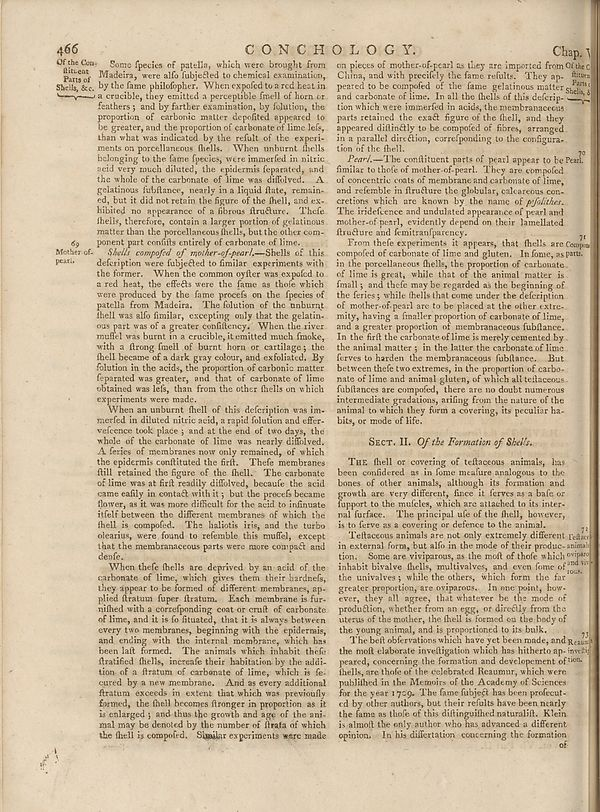
\includegraphics[width=0.85\textwidth]{../scans/page-0473-4ab88a7103cd.jpg}
\caption*{Source scan: \texttt{page-0473-4ab88a7103cd.jpg}}
\end{figure}

\end{document}
